\documentclass[../main.tex]{subfiles}
\addbibresource{../bibfile.bib}
\begin{document}
\chapter{Tecnologie utilizzate}
\label{chap:conclusion}
Questo capitolo è dedicato ad un'analisi dettagliata delle principali tecnologie adottate per lo sviluppo della piattaforma Binoculars.
Verrà approfondito il funzionamento e la struttura interna per ogni tecnologia di analisi impiegata e quali funzionalità essa offre nell'ambito dell'analisi di
file binari.
\section{Capstone}
\textit{Capstone} \cite{Capstone_docs} è una framework leggero e multi-piattaforma per effettuare il disassembly di codice macchina.
Si basa sulla famiglia di framework per compilatori \textit{LLVM}, in particolare sul modulo \textit{LLVM-Machine Code} (LLVM-MC), il quale contiene un disassemblatore interno con supporto
per molteplici architetture. Questo supporto è dato dalla presenza di molteplici \textit{tabelle descrittive} (file \textit{.TD}), le quali descrivono in maniera astratta tutte le caratteristiche
dell'ISA di una determinata architettura. 
Capstone sfrutta queste tabelle per estrarre le seguenti \textbf{informazioni semantiche}:
\begin{itemize}
    \item \textbf{Registri impliciti}: I registri letti e/o scritti \textbf{implicitamente dall'istruzione}; questi registri infatti non appaiono esplicitamente nella stringa della operazione.
    \item \textbf{Gruppi di istruzioni}: A quale categoria funzionale (es. aritmetica, logica, ...) appartiene l'istruzione
\end{itemize}
Per ogni istruzione macchina, Capstone produce una struttura dati di output denominata \textit{cs\_insn}, la quale contiene due tipi di informazioni:
\begin{itemize}
    \item \textbf{Informazioni di base (Indipendenti dall'architettura)}: ID, dimensioni (in byte), mnemonic, e una stringa contenete gli operandi dell'istruzione
    \item \textbf{Informazioni dettagliate}: Contiene le informazioni estratte dal file \textit{.TD}
\end{itemize} 
\begin{figure}[H]
    \centering
    \includegraphics[width = 0.80\textwidth]{../images/cs_isns.png}
    \caption{Struttura interna di cs\_isns. Immagine proveniente da \cite{Capstone_docs}}
\end{figure}
\section{Ghidra}
\textit{Ghidra} è un framework di reverse engineering sviluppato dalla \textit{National Security Agency} degli Stati Uniti d'America \cite{eagle2020ghidra}.
La piattaforma che il framework offre contiene un disassembler, un decompiler e un vasto insieme di tool e script di analisi. Inoltre, può essere
estesa tramite l'aggiunta di plugin e script di analisi personalizzati scritti in python o Java (il linguaggio in cui Ghidra è scritto). In particolare, è possibile interagire con le API messe a disposizione da Ghidra
direttamente da python, utilizzando la libreria \textit{pyghidra}, originariamente sviluppata dal \textit{Department of Defense Cyber Crime Center}(DC3) (un dipartimento del governo americano) e ora parte integrante della piattaforma.
L'architettura di Ghidra è estremamente complessa e formata da diversi moduli software, di cui i principali sono \cite{eagle2020ghidra}:
\begin{itemize}
    \item \textbf{Loaders}: Questi moduli si occupano dell'importazione dei file binari all'interno della piattaforma. Ogni loader è pensato per un singolo tipo di file eseguibile (ELF, Windows PE, ...). Ghidra permette inoltre di estendere
    l'insieme di loader disponibili tramite l'aggiunta di loader scritti dall'utente stesso.
    \item \textbf{Processors}: I Ghidra processors sono i moduli più complessi dell'intera piattaforma e si occupano di tutte le operazioni riguardanti il disassembly del file binario. Similmente ai file \textit{.TD} visti per Capstone, anche il processo di disassembly di Ghidra utilizza
    dei file di specifica dell'ISA per le diverse architetture supportate. Questi file sono scritti usando il linguaggio specifico per Ghidra denominato \textit{SLEIGH}.
    \item \textbf{Ghidra decompiler}: Questo modulo si occupa del processo di decompilazione del fine binario in una rappresentazione ad alto livello ispirata al linguaggio \textit{C}. Il processo di decompilazione di ghidra avviene in tre fasi distinte:
    \begin{enumerate}
        \item Il decompiler usa i file scritti in SLEIGH per creare una bozza del codice ad alto livello nel linguaggio di rappresentazione intermedia \textit{p-code}. Inoltre, in questa fase viene derivato il CFG del programma
        \item Il codice viene raffinato, eliminando gli statement irraggiungibili o inutili. A seguito di questa operazione, avviene anche una ristrutturazione del CFG in modo da riflettere i potenziali cambiamenti introdotti al flusso di controllo del programma
        \item Viene generato il codice decompilato in un linguaggio \textit{C-like}
    \end{enumerate}
\end{itemize}
\begin{figure}[H]
    \centering
    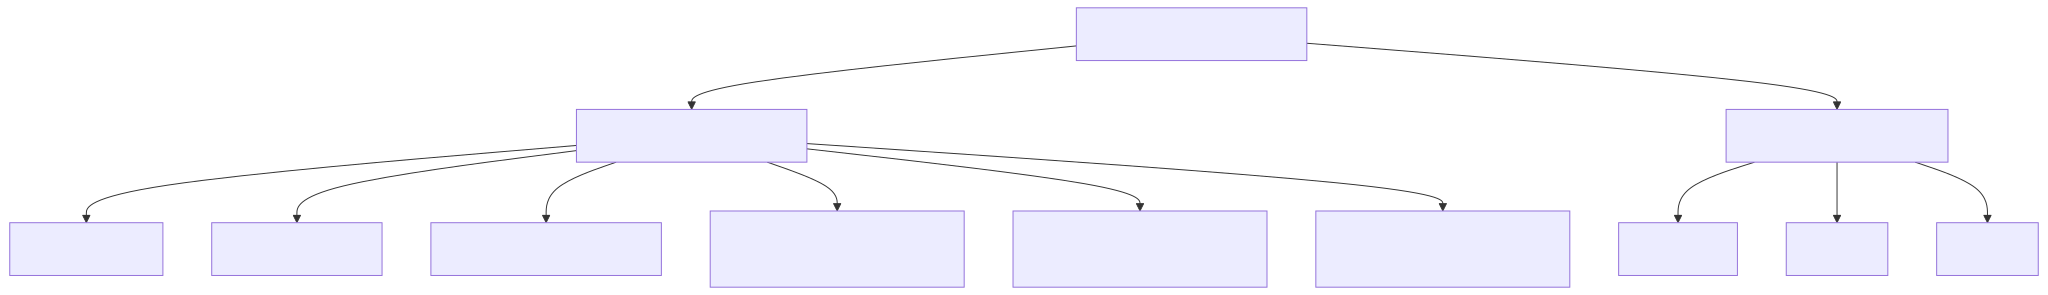
\includegraphics[width = \textwidth]{../images/ghidra.png}
    \caption{Architettura del framework Ghidra}
\end{figure}
\section{angr}
angr \cite{angr_introductory_paper} è una piattaforma per l'analisi binaria scritta in occasione della \textit{DARPA Cyber Grand Challenge 2016}.
Essa offre un supporto multi-architettura per l'esecuzione di un'ampia gamma di tecniche di analisi binaria \cite{angr_introductory_paper}:
\begin{itemize}
    \item \textbf{CFG Recovery}: angr permette di effettuare il recupero del CFG del programma caricato. Per svolgere questa funzione, angr implementa un'algoritmo iterativo per la costruzione del CFG e sfrutta una combinazione
    di tecniche di analisi per effettuare il recupero, quando possibile, degli indirizzi obbiettivo per ogni salto indiretto presente nel programma. Per ottimizzare i tempi di calcolo dell'algoritmo di recupero, angr effettua una serie di assunzioni riguardo
    al programma:
    \begin{enumerate}
        \item Tutto il codice del programma può essere distribuito in funzioni differenti.
        \item Tutte le funzioni vengono chiamate esplicitamente oppure sono precedute da un'istruzione di salto in coda.
        \item La procedura di pulizia dello stack è prevedibile e non dipende da quale funzione (chiamata o chiamante) viene invocata.
    \end{enumerate}
    \item \textbf{Value-Set Analysis}: Value-Set Analysis è una tecnica di analisi statica che permette di approssimare il valore di ogni registro e locazione di memoria ad ogni punto dell'esecuzione di un programma.
    Questa tecnica analizza il programma fino a quando l'approssimazione raggiunge un \textit{punto fisso}, cioè una sovra-approssimazione stretta di tutti i valori che ogni registro o locazione di memoria può avere ad ogni punto nel programma.
    \item \textbf{Esecuzione simbolica dinamica}: La tecnica di analisi principale messa a disposizione da angr è quella dell'analisi simbolica dinamica. La piattaforma mette a disposizione un potente motore di esecuzione simbolica, il quale sfrutta
    le funzionalità messe a disposizione dalla libreria \textit{claripy} e dal SMT solver \textit{Z3} per popolare la memoria simbolica ed effettuare il controllo di soddisfacibilità delle path condition per ogni cammino analizzato.
    \item \textbf{Under Constrained Symbolic Execution (UCSE)}: angr mette a disposizione un'ulteriore tipo di esecuzione simbolica, chiamata \textit{Under Constrained Symbolic Execution (UCSE)}. Essa effettua un'analisi separata per ogni funzione presente nel programma. Poiché ogni funzione viene analizzata senza la presenza di variabili globali e degli argomenti con cui viene chiamata, questo tipo di analisi
    non è particolarmente accurata e produce falsi positivi. UCSE etichetta tutti i dati mancanti a causa della mancanza di "contesto" (variabili globali e parametri) come \textit{under-constrained}. Quando l'analisi rileva una violazione di sicurezza, viene effettuato un controllo su tutti i valori coinvolti: se presentano tutti lo stato di \textit{under-constrained},
    allora la violazione rilevata viene filtrata come falso positivo.
    \item \textbf{Automatic Exploit Generation (AEG)}: angr mette a disposizione dei moduli per effettuare la generazione automatica di exploit, i quali permettono ad un'analista di confermare se la vulnerabilità rilevata può essere effettivamente sfruttata da un potenziale attaccante.
\end{itemize}
\newpage \noindent
La piattaforma è suddivisa nei seguenti sotto-moduli \cite{angr_introductory_paper}:
\begin{itemize}
    \item \textbf{Intermediate Representation}: Per permettere il supporto per molteplici architetture, il codice macchina del programma analizzato viene tradotto nel linguaggio di rappresentazione intermedia \textit{VEX}, sviluppato per il progetto \textit{Valgrind} e specificatamente studiato per l'analisi binaria.
    \item \textbf{CLE}: Il compito di caricare il file binario viene gestito dal modulo \textit{CLE}, acronimo ricorsivo per \textit{CLE Loads Everything}. CLE astrae il processo di caricamento per una numerosa quantità di formati di file eseguibili, gestendo la risoluzione dinamica dei simboli, la rilocazione della memoria
    e la corretta inizializzazione dello stato del programma
    \item \textbf{SimuVEX}: Il modulo \textit{SimuVEX} si occupa di effettuare la rappresentazione dello stato del programma (valori dei registri, file aperti, ...). Il modulo, inoltre, permette di rappresentare i cambiamenti semantici sullo stato del programma dati dall'esecuzione di un particolare blocco di codice. In particolare, SimuVEX permette
    di processare uno \textit{stato di input}, attraverso un blocco di codice VEX, e di generare uno \textit{stato di output} (o un'insieme di stati di output, in caso il blocco di codice contenga un'istruzione condizionale). 
    \item \textbf{Data Model}: I valori presenti nei registri sono rappresentati tramite le astrazioni messe a disposizione dalla libreria \textit{Claripy}. 
    La libreria astrae ogni valore in una rappresentazione simbolica chiamata \textit{espressione}, la quale traccia tutte le operazioni in cui essa viene utilizzata.
    Le espressioni vengono rappresentate mediante strutture ad albero chiamate \textit{expression trees}, nelle quali i nodi intermedi contengono l'operazione svolta, mentre le foglie contengono i valori usati come argomenti dell'operazione.
    Per esempio, se all'espressione $x$ viene aggiunta l'espressione $5$, la nuova espressione risultante sarà $x+5$. Il suo \textit{expression tree}, quindi, avrà l'operazione di somma alla radice, mentre le foglie conterranno le espressioni $x$ e $5$.
    \item \textbf{Full program analysis}: Questo modulo mette a disposizione dell'analista un entry point (la classe \textit{Project}) per accedere sia alle funzionalità dei moduli descritti sopra sia alle tecniche di analisi binaria messe a disposizione dalla piattaforma.
\end{itemize}
\begin{figure}[H]
    \centering
    \includegraphics[width = 0.40\textwidth]{../images/angr_architecture.png}
    \caption{Architettura di angr. Immagine proveniente da \cite{angr_architecture}}
\end{figure}
\end{document}